%
% File naacl2019.tex
%
%% Based on the style files for ACL 2018 and NAACL 2018, which were
%% Based on the style files for ACL-2015, with some improvements
%%  taken from the NAACL-2016 style
%% Based on the style files for ACL-2014, which were, in turn,
%% based on ACL-2013, ACL-2012, ACL-2011, ACL-2010, ACL-IJCNLP-2009,
%% EACL-2009, IJCNLP-2008...
%% Based on the style files for EACL 2006 by 
%%e.agirre@ehu.es or Sergi.Balari@uab.es
%% and that of ACL 08 by Joakim Nivre and Noah Smith

\documentclass[11pt,a4paper]{article}
\usepackage[hyperref]{naaclhlt2019}
\usepackage{times}
\usepackage{latexsym}
\usepackage{url}
\usepackage{multirow}
\usepackage{graphicx}
\usepackage{amssymb}
\usepackage{amsmath}
\usepackage{CJKutf8} 

\aclfinalcopy % Uncomment this line for the final submission
%\def\aclpaperid{***} %  Enter the acl Paper ID here

%\setlength\titlebox{5cm}
% You can expand the titlebox if you need extra space
% to show all the authors. Please do not make the titlebox
% smaller than 5cm (the original size); we will check this
% in the camera-ready version and ask you to change it back.

\newcommand\BibTeX{B{\sc ib}\TeX}

\title{Naive Bayes and BiLSTM Ensemble for Discriminating between Mainland and Taiwan Variation of Mandarin Chinese}

\author{Li Yang \\
  Tongji University \\
  Shanghai \\
  China \\
  {\tt li.yang@tongji.edu.cn} \\\And
  Yang Xiang \\
  Tongji University \\
  Shanghai \\
  China \\
  {\tt shxiangyang@tongji.edu.cn} \\}

\date{}

\begin{document}
\maketitle
\begin{abstract}
  Automatic dialect identification is a more challenging task than language identification, requiring ability to discriminate between different varieties within the same language family. In this paper, we propose an ensemble based system, which combine traditional machine learning models trained on bag of n-gram fetures, with deep learning models trained on word embeddings, to solve the Discriminating between Mainland and Taiwan Variation of Mandarin Chinese (DMT) shared task at VarDial 2019. Our experiments show that a character bigram-trigram combination based Navie Bayes is a very strong model for identifying varieties of Mandarin Chinense. By combining Navie Bayes and BiLSTM using average ensembling, a simple yet effective approach, our system achived an macro-averaged F1 acore of number1\% and number2\% in two tracks, ranking th and th out of number teams respectively.
\end{abstract}

\section{Introduction\label{introduction}}

Dialect identification can be considered as a specical case of language identification, which aims at distinguishing  related languages or varieties of a specific language. Being capable of detecting dialect accurately is an important step for many NLP piplines and applications, such as automatic speech recognition, machine translation and multilingual data acquisition. While language identification can already achieve relatively high performance with a simple model, dialect identification is still a tough problem remained to be tackled. In contrast to the language identification scenario, the linguistic difference between related languages is less obvious. For that reason, dialect identification has drawn many researchers' attention in recent years, becoming an important and attractive research topic.

\begin{table}[t!]
\begin{center}
\begin{tabular}{ccc}
\hline \bf Term & \bf Mainland China & \bf Taiwan \\ \hline
taxi & \begin{CJK}{UTF8}{gbsn}出租车\end{CJK}  &  \begin{CJK}{UTF8}{bsmi}計程車\end{CJK} \\
bicycle &   \begin{CJK}{UTF8}{gbsn}自行车\end{CJK} & \begin{CJK}{UTF8}{bsmi}腳踏車\end{CJK} \\
softmax & \begin{CJK}{UTF8}{gbsn}软件\end{CJK} &  \begin{CJK}{UTF8}{bsmi}軟體\end{CJK}  \\
program &  \begin{CJK}{UTF8}{gbsn}程序\end{CJK} & \begin{CJK}{UTF8}{bsmi}程式\end{CJK} \\
kindergarten &  \begin{CJK}{UTF8}{gbsn}幼儿园\end{CJK} & \begin{CJK}{UTF8}{bsmi}幼稚園\end{CJK} \\
\hline
\end{tabular}
\end{center}
\caption{\label{vocab differ} Different expressions with the same meaning used in Mainland China and Taiwan. }
\end{table}

Mandarin Chinese is a group of related varieties of Chinese spoken across many different regions. The group includes \textit{Putonghua}, the offical language of Mainland China, and \textit{Guoyu}, another Mandarin variant widely spoken in Taiwan. However related they are, there are still some difference between these two varieties. First, the most notable one is the character set they use. Mainland Chinese uses simplified Chinese characters, as opposed to the traditional Chinense characters for Taiwanese Chinese. Take the phrase ``\textit{natural language processsing}'' as an example, its simplified character form adopted in Mainland China is ``\textit{\begin{CJK}{UTF8}{gbsn}自然语言处理\end{CJK}}'', while the traditional character form in Taiwan is ``\textit{\begin{CJK}{UTF8}{bsmi}自然語言處理\end{CJK}}". Second,  some vocabularies differ. There are some terms can be understood by both varieties to mean the same thing. However, their preferred usage distinguishes. Table~\ref{vocab differ} lists some examples. Apart from character form and vocabularies, the pronunciation escpecially in terms of tone is also different. But we don't discusss in this paper since it's less relevant.

The DMT task, first introduced by VarDial evaluation campagin this year, aimming at determining whether a sentence belongs to news articles from Mainland China or from Taiwan. The organizers prepare two versions of the same corpus, traditional and simplified, and ask participants to predict the labels for text instances in both tracks.  For that reason, one can't make use of character form to discriminate these two language varieties. Mainstream approaches to dialect identification is to regard it as a text classification task and use a linear support vector machine (SVM) with bag of n-gram features as input to slove it. However, we want to know what's the best classification algorithm for DMT task. Therefore, we experiment with serveral classical machine learning models trained on different word or character level n-gram features and feature combinatons. Besides, deep learning methods have currently achieve remakable sucess in many NLP tasks, including question answering~\cite{DBLP:journals/corr/FengXGWZ15}, sentiment analysis~\cite{D17-1047}, machine translation~\cite{NIPS2017_7181} and natural language inference~\cite{ACLP17-1152}. To inverstigate how much can deep neural neworks help identify language varieties, we test 7 different deep learning models, varying from CNN based, RNN based to CNN-RNN hybrid models. Fully performance comparison to machine learning models is alos conducted. Finally, we explore different ways to combine the classifiers we discuss before.

The rest of this paper is organized as follows. Section~\ref{related work} introduces related work. In Section~\ref{data and methodlogy}, we describe the dataset and our proposed solution. Experimental results are presented in Section~\ref{experiments}, and we give our conclusion and feature work in Section~\ref{conclusion and feature work}.

\section{Related work\label{related work}}
A number of works have devoted to identify different language varieties or related language, especially since the series of VarDial evaluation campaigns~\cite{W16-4801, W17-1201, W18-3901}.~\cite{U13-1003}~studies on English dialect identification and presents serveral classification approaches to classify Australia, British and Caniadian English. \cite{Zampieri2012AutomaticIO} utilizes a character n-gram and a word n-gram language model for automatic classificaton of two written varieties of Portuguese: European and Brazilian. \cite{Ciobanu2016ACP}~conducts an intial study on the dialects of Romanian and proposes using the orthographic and phonetic features of the words to build a dialect classifier. \cite{W17-1221} uses a majority-vote ensemble of the Navie Bayes, CRF and SVM systems for Swiss German dialects identification. \cite{W18-3922} uses two SVM classifiers: one trained on word n-grams fewtures and one trained on Pos n-grams to determine a document to be in Flemish Dutch or Netherlandic Dutch. \cite{W18-3906} uses a unified SVM model based on character and word n-grams features with careful hyperparameter tuning for 4 language/dialect identification tasks.

Methods to discriminate between varieties of Mandarin Chinese haven't been well studied. \cite{Y08-1042} uses a top-bag-of-word similarity based contrastive approach to reflect distance among three varieties of Mandarin: Mainland China, Singapore and Taiwan. \cite{IJNLC2016:5} deals with 6 varieties of Mandarin: Maninland, Hong Kong, Taiwan, Macao, Malaysia and Singapore. They discovers that character bigram and word segmentation based feature work better than traditional character unigram, and some features such as character form, PMI-based and word alignment-based features can help improve performance. However, a thorough comparison of different algorithms and architectures has yet to be conducted.

\section{Data and Methodology\label{data and methodlogy}}

\begin{table*}[]
\centering
\begin{tabular}{cccclcccc}
\hline
\multirow{2}{*}{\textbf{Variety}} & \multicolumn{3}{c}{\textbf{Number of instances}} &                      & \multicolumn{4}{c}{\textbf{Sentence length}} \\ \cline{2-4} \cline{6-9} 
                                  & train           & valid          & test          & \multicolumn{1}{c}{} & min      & max      & avg      & st.dev.     \\ \hline
Mainland China                    & 9385            & 1000           & 1000          &                      & 5        & 66       & 9.63     & 3.73        \\
Taiwan                            & 9385            & 1000           & 1000          &                      & 6        & 48       & 9.24     & 3.30        \\ \hline
\end{tabular}
\caption{Statistics of dataset for each variety. Sentence lengths are calculated based on word-level tokens from training and validation set.}
\label{data staticstics}
\end{table*}

\subsection{Data\label{data}}
The DMT task is provided with labeled sentences belonging to news articles from Mainland China or from Taiwan, which compose of 18770 instances for training set, 2000 for validation set and 2000 for test set. As shown in Table~\ref{data staticstics},  the DMT dataset has a perfectly balanced class distribution. The avergae sentence length (in word level) of two varieties are almost the same, and short as well. It's worth mentioning that the organizers have prepared two version of the same dataset: traditional and simplified version, which means we can't utilize character form feature to help us discriminate between these two language variety.  Since the sentences have been tokenized and punctuation removed from the texts, we don't apply any preprocessing on the dataset.

\subsection{Machine Learning Models with n-gram features\label{ml models}}
Machine learning models based on feature engineering are the most common methods for dialect identification. In this paper, we experiment with 3 different classifiers: (1) logistic regression (\textbf{LR}), (2) linear support vector machine (\textbf{SVM}), and (3) multinomial Naive Bayes (\textbf{MNB}) based on bag of n-gram features. We also examine other Navie Bayes models such as Gaussian Navie Bayes and Bernoulli Naive Bayes, but they are inferior to multinomial Naive Bayes on the validation set. The bag of n-gram features include word and character level n-gram with size ranging from unigram to n-gram of specific order. We conduct a set of experiments to fully explore the most contributing features and feature cobinations for DMT task, and the results are shown in next Section.

\subsection{Deep Learning Models with word embeddings\label{dl models}}
\begin{figure}
\centering
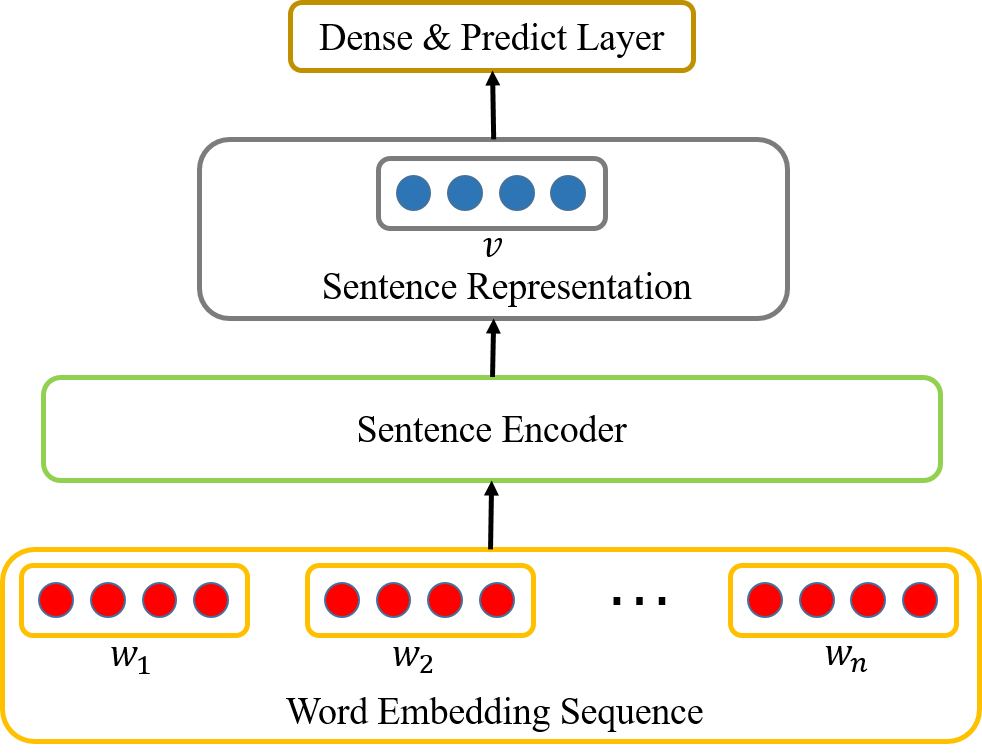
\includegraphics[scale=0.35]{framework.png}
\caption{The overall framework of deep models.}
\label{framework}
\end{figure}
Deep neural networks (DNNs) are of growing interest for their capacity to learn text representation from data without careful engineering of features.  For short-text classification task, Convolution neural network (CNN) and recurrent neural network (RNN) are two mainstream DNN architectures. In this paper, we examine a number of deep models based on the same framework to solve DMT task. Figure~\ref{framework} shows a high-level view of the framework. Vertically, the figure depicts 3 major components: (1) \textbf{Input Embedding Layer}. Suppose the sentence has \textit{n} tokens, we use a pre-trained embedding method Word2vec~\cite{DBLP:journals/corr/abs-1301-3781} based on training data to represent it in a sequence of word embeddings:
\begin{equation} 
S=\left(\mathbf{w}_{\mathbf{1}}, \mathbf{w}_{\mathbf{2}}, \cdots \mathbf{w}_{\mathbf{n}}\right)
\end{equation}
where $w_i$ is a vector representing a $d$ dimentional word embedding for the $i$-th word in the sentence. $S$ is thus a sequence that concatenates all word embeddings together. We do try using character embeddings as input and other pre-trained embedding methods such as Glove~\cite{pennington2014glove} and Fasttext~\cite{bojanowski2017enriching} but observed no further improvement on validation set. (2) \textbf{Sentence Encoder Layer}. Sentence encoder, specified by different deep models, processes the input word embedding sequence and output a sentence representation: 
\begin{equation} 
v=encode\left(S\right)
\end{equation}
(3) \textbf{Output Layer}. After obtaining sentence vector, we feed it through one hidden dense layer with 256 unit and a final predict dense layer:
\begin{equation} 
 \hat{y}=\sigma\left(\mathbf{W_{p}} \gamma\left(\mathbf{W_{h}} v+\mathbf{b_{h}}\right)+\mathbf{b_{p}}\right)
 \end{equation} 
  where $\mathbf{W_{h}}$ and $\mathbf{b_{h}}$ are the parameters for hidden layer, $\mathbf{W_{p}}$ and $\mathbf{b_{p}}$ are the parameters for predict layer, $\gamma$ and $\sigma$ are relu and sigmoid activation function respectively, $\hat{\mathbf{y}} \in \mathbb{R}$ represents the predicted score for postive class. During traing process, we minimize the binary cross-entropy loss defined as follow:
\begin{equation} 
L=-\frac{1}{N} \sum_{i=1}^{N}\left(y_{i} \log \hat{y}_{i}+\left(1-y_{i}\right) \log \left(1-\hat{y}_{i}\right)\right)
\end{equation}
 where $y_{i}$ is the ground-truth.

We compare 7 different deep models to encode sentence into fixed-size vector, including cnn-based, rnn-based and cnn-rnn hybird neural networks.
\begin{itemize}
        \item \textbf{CNN:} First introduced by \cite{D14-1181}, the convolution network applies a concolution operation with a filter $\mathbf{W_{c}} \in \mathbb{R}^{h d}$ to a window of h words to produce a new feature.
        \begin {equation} 
	 c_{i}=f\left(\mathbf{W_{c}} \cdot \mathbf{x}_{i : i+h-1}+b\right)
 	\end {equation}
By applying this filter to each possible window of words in the sentence, a feture map can be produced. In this paper, we use 300 filters with size ranging from 2 to 5 to extract four 300 dimensional feature maps.  After that, we apply max-over-time pooling operation by taking the highest value for each feature map to capture the most important feature, then concatanate all the feature to represent the input sentence.
        \item \textbf{DCNN:} \cite{P14-1062} use a dynamic convolution neural network (DCNN) that alternates wide concolution layers and dynamic $k$-Max pooling layers for sentence modeling. By applying $k$-Max pooling operation, a feature graph over the sentence can be induced, being capable of explicitly capturing both short and long-range relations.
        \item \textbf{DPCNN:} \cite{P17-1052} propose a deep concolutional neural network by stacking concolution blocks (two concolution layers and a shortcut connection) interleaved with pooling layers with stride 2 for downsampling. The 2-stride downsampling reduces the size of the internal represenation of each text by half, enabling efficient representation of long-range association in the text.  And the shortcut connection ensure training of deep networks. DPCNN has been shown powerful in many text classificaiton task.
        \item \textbf{BiLSTM:} LSTM is an effective neural network for sentence modeling for its ability to capture long-term dependencies. BiLSTM use a forward and a backward LSTM to process sequence, such that each produced hidden state can contain information from context in two opposite direction. Specifically, at each time step $t$, hidden state $h_{t}$ is the concatenation of results from forward and backward LSTM:
\begin{equation}
\begin{aligned}
  		\overrightarrow{h_{t}}&=\overrightarrow{\mathrm{LSTM}}\left(\mathbf{w_{1}}, \mathbf{w_{2}}, \ldots, \mathbf{w_{t}}\right)    \\
  		\overleftarrow{h_{t}}&=\overleftarrow{\mathrm{LSTM}}\left(\mathbf{w_{n}}, \mathbf{w_{n-1}}, \ldots, \mathbf{w_{t}}\right)     \\
  		 h_{t}&=\left[\overrightarrow{h_{t}}, \overleftarrow{h_{t}}\right]
  	\end{aligned}
\end{equation}	
After obtaining hidden state squence, we apply max-over-time pooling operation to form a fixed-size vector as sentence representation $v$.
	\item \textbf{Self-attentive BiLSTM:} Attention mechanism is most comonly used in sequence-to-sequence models to attend to encoder states~\cite{DBLP:journals/corr/BahdanauCB14, DBLP:journals/corr/VaswaniSPUJGKP17}. In this paper, we make use of attention, more specifically, self-attention~\cite{DBLP:journals/corr/LinFSYXZB17} to obtain a distribution over features learned from BiLSTM (a.k.a hidden states). Suppose $H$ is the output hidden vectors of BiLSTM: $H=\left(\mathbf{h}_{\mathbf{1}}, \mathbf{h}_{\mathbf{2}}, \cdots \mathbf{h}_{\mathbf{n}}\right)$, we can calculate the attention vector $\alpha$ and the final sentence representation $v$ as follows:
\begin{equation}
\begin{aligned}
  		e_{t}&=\mathbf{U}_{a}^{\top} \tanh \left(\mathbf{W}_{a} \mathbf{h}_{t}\right)    \\
  		\alpha_{t}&=\frac{\exp \left(e_{t}\right)}{\sum_{i=1}^{T} \exp \left(e_{i}\right)}     \\
  		 v&=\Sigma_{i=1}^{T} \alpha_{i} h_{i}
\end{aligned}
\end{equation}
where $\mathrm{W}_{a} \in \mathbb{R}^{2d \times 2d}$ and $\mathrm{U}_{a} \in \mathbb{R}^{2d \times 1}$ are parameters of attention layer (we use $d$ units for LSTM, thus ${h_{t}}$ is a $2d$ dimensional vector).  Using self-attention allows sentence to attend to itself, thus we can extract the most relevant information.
	\item \textbf{CNN-BiLSTM:} Similar as \cite{DBLP:journals/corr/ZhouSLL15b}, we first use CNN to extract a higher-level sequence representation from word embedding sequence, and then feed them into BiLSTM to obtain final sentence representation. By combing CNN and BiLSTM, we are able to capture both local features of phrases and global informantion of sentence. 
	\item \textbf{BiLSTM-CNN:} We also try to use the BiLSTM layer as feature extrator first and then eed the hidden states to the CNN layer, which we call BiLSTM-CNN.
\end{itemize}

\subsection{Ensemble Models\label{ensemble models}}
Classifier ensembles are a way of combining different models with the goal of improving overall peformance through enhanced decision making, which has been shown to achieve better results than single classifier. In this paper, we explore 4 ensemble strategies to intergrate output (predict label or probability) from models introduced above and reach a final decision.
\begin{itemize}
	\item \textbf{Mean Probability:}  Simply take an average of predictions from all the models and use it to make the final prediction.
	\item \textbf{Highest Confidence:} The class label that recieves vote with the highest probability is selected as the final prediction.
	\item \textbf{Majority Voting:} Each classifier votes for a single class label. The votes are summed and the label with majority votes (over 50\%) wins. In case of tie, the ensemble result falls back to the prediction by the model with highest peformance on validation set.
	\item \textbf{Meta-Classifier:} Use the individual classifier outputs along with training labels to train a second-level meta-classifier.The second meta-classifier then servers to predict the final prediction. Meta-Classifier is also refered to as classifier stacking.
\end{itemize}

While the first three strategies use a simple fusion method to combine models, Meta-Classifier has parameters to train, which attempts to learn the collective knowledge represented by base classifiers. As for choosing estimator for meta-classfier, we test with a wide range of learning algorithms including not only the ones mentioned in Section\ref{ml models}, such as random forest, GBDT and XGBoost. It turns out Gaussian Navie Bayes is the most competitive model, which will be the only meta classifer discusssed in next Section.

\section{Experiments\label{experiments}}
\subsection{Experimental setup}
We use scikit-learn library\footnote{https://scikit-learn.org/stable/} for implementation of the n-gram features based models and the ensemble meta-classifier. As for deep models, we implement them using Keras\footnote{https://github.com/keras-team/keras} library with Tensorflow backend. We used Adam~\cite{DBLP:journals/corr/KingmaB14} method as the optimizer, setting the first momentum to be 0.9 , the second momentum 0.999 and the initial learning 0.001. The bacth size is 32. All hidden states of LSTMs, feature maps of CNNs and word embeddings have 300 dimensions. Word embeddings are fine tuned during training process. All  the models are trained separately on traditional and simplified version's dataset, and evaluated using macro-weighted f1 score. Our code for all experiments is publicly available\footnote{https://github.com/AlexYangLi/DMT}. 

\begin{figure*}
\centering
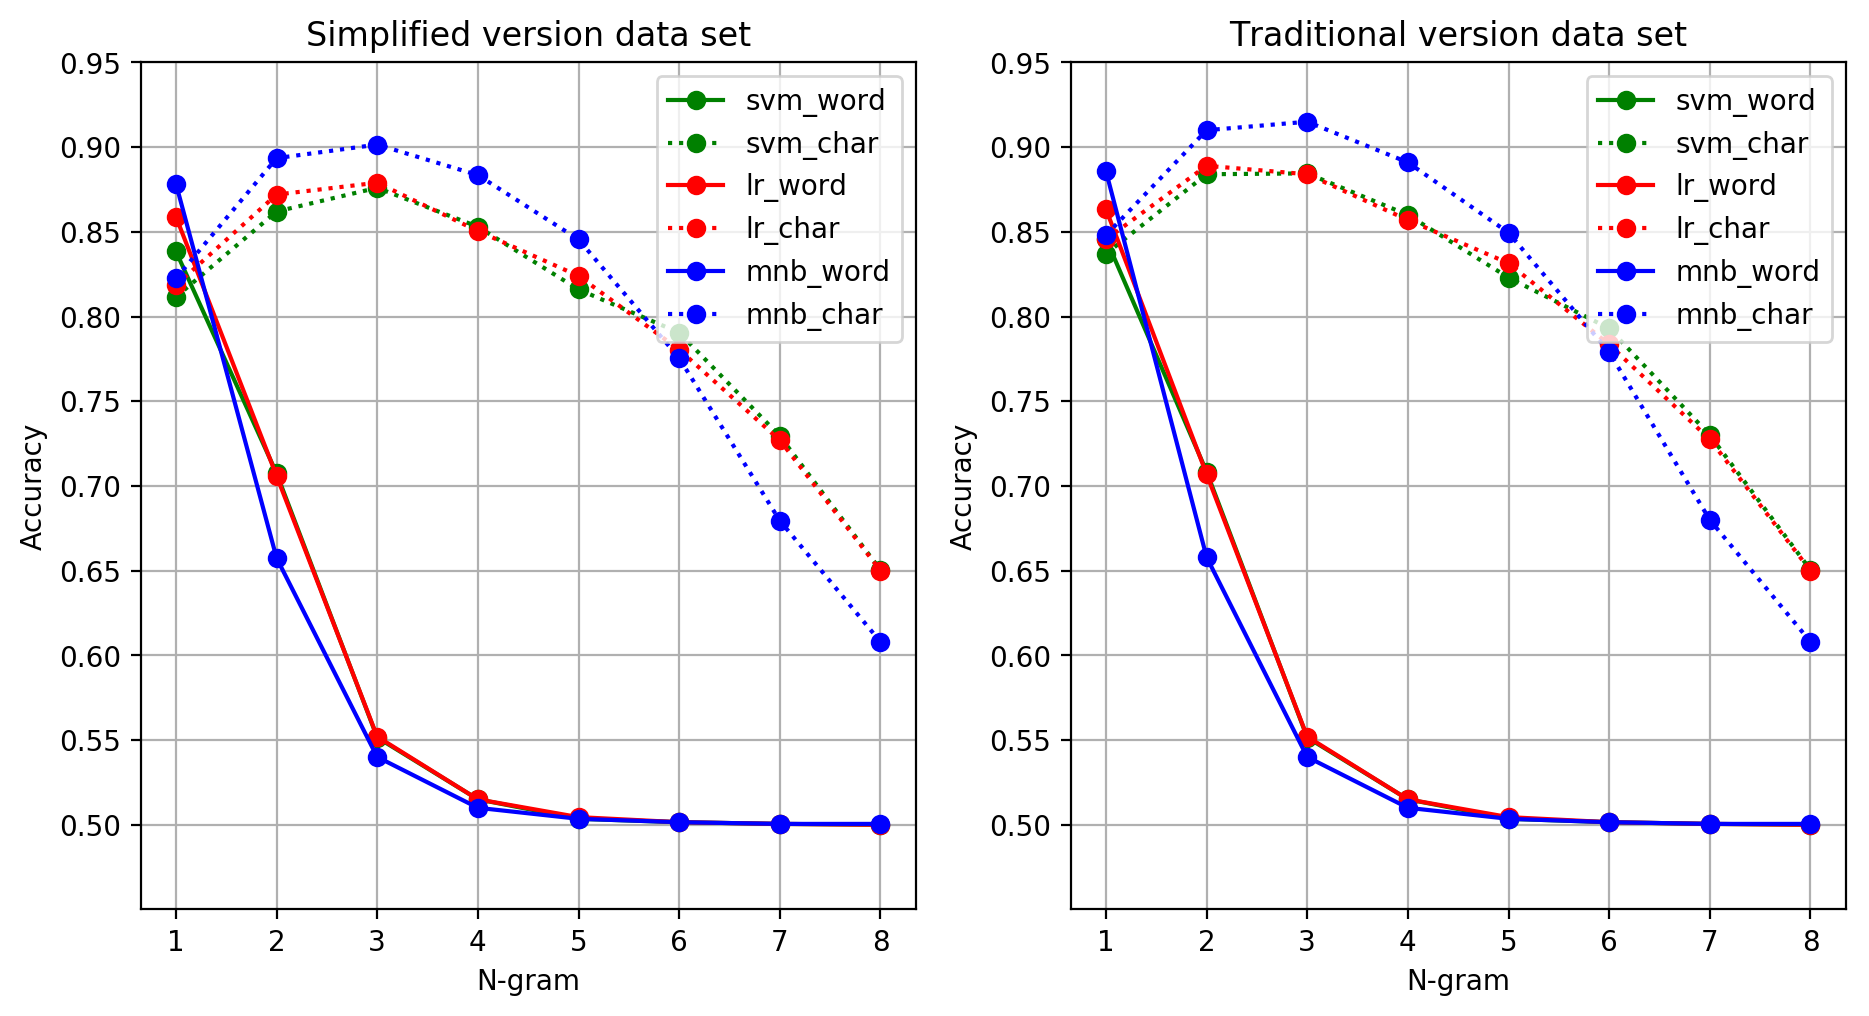
\includegraphics[scale=0.6]{single_n_gram_1_2.png}
\caption{Macro-weighted f1 scores for LR (red lines), SVM (green lines), MNB (blue lines) using character (solid lines) or word level (dotted lines) n-gram of different sizes as input, both on dataset of simplified (left) and traditional (right) version.}
\label{single_ngram_p}
\end{figure*}

\begin{table*}[]
\begin{tabular}{lccclccc}
\hline
\multirow{2}{*}{\textbf{Feature}}     & \multicolumn{3}{c}{\textbf{Simplified}} &  & \multicolumn{3}{c}{\textbf{Traditional}} \\ \cline{2-4} \cline{6-8} 
                                      & LR       & SVM      & MNB               &  & LR        & SVM      & MNB               \\ \hline
\multicolumn{8}{l}{\textbf{Individual feature}}                                                                               \\
word uigram                           & 0.8590   & 0.8384   & 0.8784            &  & 0.8634    & 0.8460   & 0.8860            \\
char bigram                           & 0.8720   & 0.8620   & 0.8935            &  & 0.8890    & 0.8840   & 0.9100            \\
char trigram                          & 0.8790   & 0.8760   & 0.9015            &  & 0.8840    & 0.8845   & 0.9150            \\
char 4gram                            & 0.8504   & 0.8474   & 0.8835            &  & 0.8570    & 0.8559   & 0.8910            \\ \hline
\textbf{Combined feature}             &          &          &                   &  &           &          &                   \\
char bigram+trigram                   & 0.8865   & 0.8830   & \textbf{0.9080}   &  & 0.8960    & 0.8925   & \textbf{0.9225}   \\
char bigram+trigram+4gram             & 0.8880   & 0.8835   & 0.9030            &  & 0.8945    & 0.8920   & 0.9170            \\
char bigram+char trigram+word unigram & 0.8875   & 0.8835   & 0.9055            &  & 0.8990    & 0.8940   & 0.9200            \\ \hline
\end{tabular}
\caption{Macro-weighted f1 scores for LR, SVM, MNB using individual or combined features as input, both on dataset of simplified and traditional version.}
\label{combine_ngram_p}
\end{table*}

\begin{table*}[]
\begin{center}
\begin{tabular}{lcc}
\hline
\textbf{Model}  & \textbf{Simplfied} & \textbf{Traditional} \\ \hline
\multicolumn{3}{l}{\textbf{CNN-based}}          \\
CNN                   & 0.8964    & 0.9090       \\
DCNN                  & 0.8970     & 0.9080       \\
DPCNN                 & 0.8925    & 0.9070       \\ \hline
\multicolumn{3}{l}{\textbf{RNN-based}}          \\
BiLSTM                & \textbf{0.9000}       & \textbf{0.9115}      \\
Self-attentive BiLSTM & 0.8915    & 0.9020       \\ \hline
\multicolumn{3}{l}{\textbf{CNN-RNN hybrid}}     \\
CNN-BiLSTM            & 0.8935    & 0.9080       \\
BiLSTM-CNN            & 0.8950     & 0.9095      \\ \hline
\end{tabular}
\caption{Macro-weighted f1 scores for deep models using word embeddings as input, both on dataset of simplified and traditional version.}
\label{dl_model_p}
\end{center}
\end{table*}

\begin{table*}[]
\begin{center}
\begin{tabular}{lccclccc}
\hline
\multirow{4}{*}{\textbf{Ensemble Strategy}}           & \multicolumn{3}{c}{\textbf{Simplfied}}                                                        &  & \multicolumn{3}{c}{\textbf{Traditional}}                                                      \\ \cline{2-4} \cline{6-8} 
                   & all ML$^*$ & all DL$^*$ & \begin{tabular}[c]{@{}c@{}}MNB \\ + \\ BiLSTM\end{tabular} &  & all ML$^*$ & all DL$^*$ & \begin{tabular}[c]{@{}c@{}}MNB \\ + \\ BiLSTM\end{tabular} \\ \hline
Mean Probability   & 0.9025     & 0.9050     & \textbf{0.9130}                                            &  & 0.9170     & 0.9215     & \textbf{0.9240}                                            \\
Highest Confidence & 0.9080     & 0.9015     & \textbf{0.9130}                                            &  & 0.9225     & 0.9100     & \textbf{0.9240}                                            \\
Majority Voting    & 0.8880     & 0.9060     & -                                                          &  & 0.8985     & 0.9195     & -                                                          \\
Meta-Classifier    & 0.8915     & 0.9025     & 0.9050                                                     &  & 0.906      & 0.9130     & 0.9215                                                     \\ \hline
\end{tabular}
\caption{Macro-weighted f1 scores for 4 ensemble strategies combining different base classifiers, both on dataset of simplified and traditional version. ``all ML'' and ``all DL'' refer to combine all machine learning models and deep learning models respectively. All machine learning models use character bigram-trigram combination as input.}
\label{ensemble_model_p}
\end{center}
\end{table*}

\subsection{Contribution of single n-gram features}
To find the most contributing individual n-gram features for discriminating Mandarin Chinese varieties. We run a number of experiments with the three classifiers using one single n-gram at a time, and the results are illustrated  in Figure~\ref{single_ngram_p}. As we can see, for dataset of both simplified and traditional version, performances of 3 models all drop sharply when using a n-gram of larger size, especially for word level n-grams. The most contributing character level ngram is character trigram, to which character bigram is inferior yet close. Word unigram is the best between word level n-grams, but no better than character bigram or trigram. Among all 3 models, MNB outperforms LR and SVM, despite the trend that SVM has been the most preferred method for dialect identification. Besides, we can also see from the figure that performances on dataset of traditional version are slightly better than simplified version, which is persist with different models.

\subsection{Combination of n-gram features}
Table~\ref{combine_ngram_p} shows the results of combining individual feature on each dataset. The performances of individual feature are also listed for direct comparison. As indicated from the table, feature combination does bring a performance gain. While 3 kinds of combination achieve a close score, MNB using combination of character bigram and trigram is the best, achiving macro-weighted f1 score of 0.9080 for simplfied version dataset and 0.9225 for traditional version.

\subsection{Performance of deep learning models}
To fully compare deep learning methods with machine learning methods for DMT task, 7 deep models are evaluated. Results are listed in Table~\ref{dl_model_p}. Among 7 deep models, BiLSTM stands out from the others with macro-weighted score of 0.9000 and 0.9115. All deep models outperform LR and SVM, but are inferior to MNB, which shows again MNB is a very strong classifier for discriminating variations of Mandarin Chinese.

\subsection{Performance of ensemble models}
We also try to achieve a better result by aggregating the outputs of models we have implemented. As presented in Table~\ref{ensemble_model_p}, no single ensemble strategy performs consistenly better than the others. The best choice for ensemble model is using MNB and BiLSTM as base classifier, and Mean Probability or Highest Confidence as fusion method. (When there are only 2 base classifiers, results of Mean Probability and Highest Confidenceare are always the same.)

\subsection{Results of shared task}
To do.

\section{Conclusion and feature work\label{conclusion and feature work}}
To do.

\bibliography{dmt}
\bibliographystyle{acl_natbib}

\end{document}
